\documentclass[UTF8]{EPURapport}
%\usepackage{listings}

%\renewcommand{\lstlistlistingname}{Liste des codes}
%\renewcommand{\lstlistingname}{Code}

%\addextratables{%
%	\lstlistoflistings
%}

%\swapAuthorsAndSupervisors

\thedocument{Manuel utilisateur}{Canne connectée pour aveugles}{}
\grade{Département Informatique\\ 5\ieme{} année\\ 2020-2021}
\authors{%
	\category{Auteurs}{%
		\name{Djawad M'DALLAH MARI} \mail{djawad.mdallah-mari@etu.univ-tours.fr}
	}
	\details{DII5 2020-2021}
}
\supervisors{%
	\category{Encadrants}{%
		\name{Gilles VENTURINI} \mail{gilles.venturini@etu.univ-tours.fr}
	}
	\details{Université François-Rabelais, Tours}
}
\abstracts{Manuel utilisateur canne connecée pour aveugles}
{}
{}
{}

\begin{document}

\chapter{Introduction}

Ce document fait partie d'un ensemble de livrables qui accompagne le projet de fin d'études "Canne connectée pour aveugles" réalisé en 2020-2021 à Polytech Tours par Djawad M'DALLAH-MARI.\\

C'est le manuel utilisateur qui vise toute personne souhaitant utiliser l'application et connaître les différentes fonctionnalitées proposées.

\chapter{Prérequis et installation}

L'application a été développée et compilée avec l'\verb|API level 28| c'est-à-dire \textbf{Android 9}. L'application peut fonctionner sur des versions antérieures, mais peut présenter des anomalies.
Pour une utilisation optimale, \textbf{il est conseillé d'avoir un smartphone Android avec une version égale ou supérieur à Android 9}. \\

Dans le cadre où l'application a été déployée sur le Google Play, le moyen le plus facile pour un utilisateur d'installer l'application est de le télécharger directement sur le Google Play.\\

Si l'application n'est pas déployée sur le Google Play, il faudra se procurer directement le fichier APK. La dernière version de l'APK déployée est disponible sur le github du projet \footnote{\url{https://github.com/Djawad-mdallahmari/PFE-ObjectDetection/tree/master/apk}}. Une fois téléchargé, il suffit de le transférer sur le smartphone et cliquer dessus pour l'installer. Veillez à activer l'option permettant d'installer des applications à partir de sources inconnues \footnote{Option disponible dans Paramètres > Sécurité}.

\chapter{Les fonctionnalités}

\section{Détection d'objets}

La fonctionnalité principale est la détection et l'identification d'un objet. Cette fonction utilise l'appareil photo arrière du smartphone pour capturer l'image renvoyée puis identifie les objets. Aucune configuration au préalable n'est requise pour activer cette fonctionnalité. Il suffit donc de pointer son appareil sur les objets à détecter pour utiliser cette fonctionnalité.

\begin{figure}[h!]
\centering
  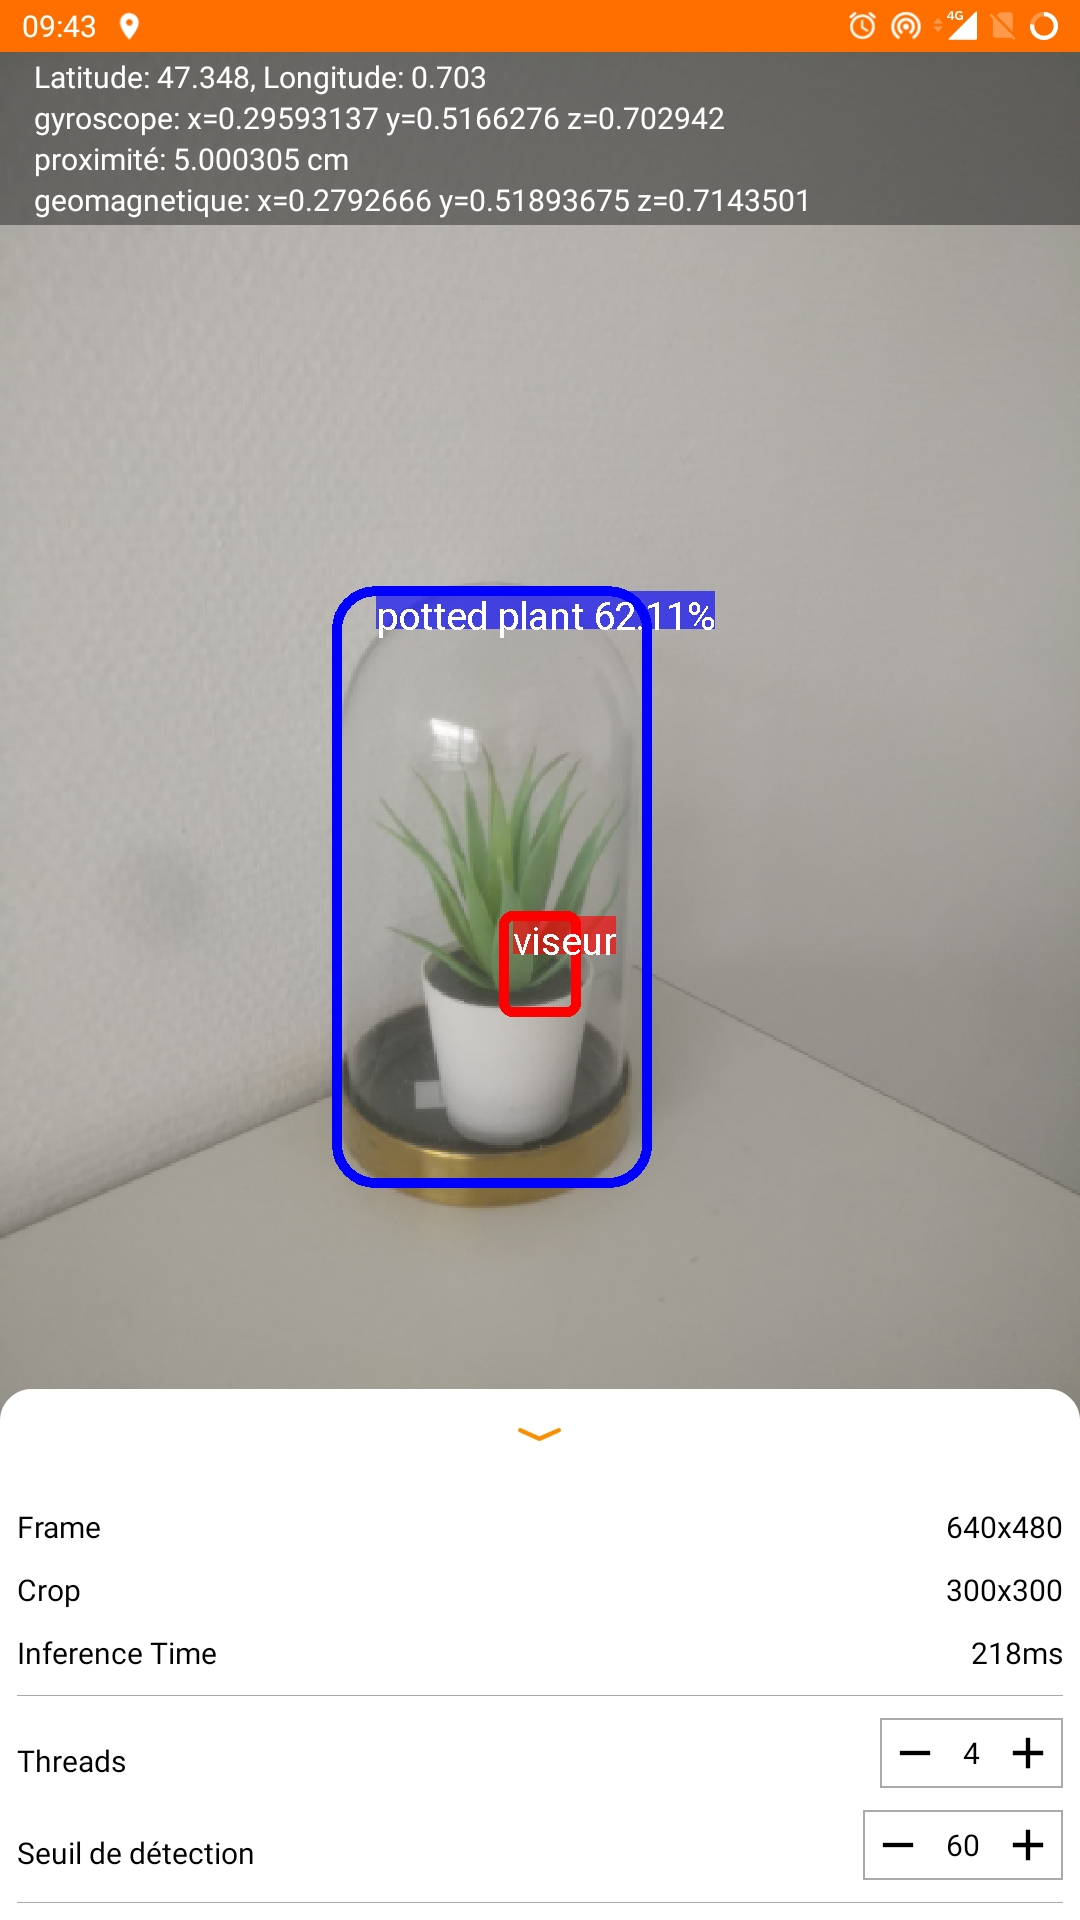
\includegraphics[width=0.3\textwidth]{images/result.jpg}
  \caption{Détection d'objet}
  \label{fig:objectdetection}
\end{figure}
\section{Retour sonore}

Destinée aux personnes malvoyantes, l'une des fonctionnalités majeures également est le retour sonore. En effet, l'application utilise la synthèse vocale pour énoncer le nom des objets détectés. Cette fonctionnalité est déjà activée par défaut donc aucune configuration n'est requise pour pouvoir profiter de cette fonctionnalité. L'application énoncera automatiquement chaque objet détecté.\\

Il existe une fonction de \textbf{Mute} permettant de rendre le synthétiseur vocal muet. Cette fonction peut être activée en cliquant une fois sur l'écran. Pour le réactiver, il suffit de recliquer une nouvelle fois.\\

Dans le cadre où le Mode Assistant par défaut du smartphone est activé, il est toujours possible de bénéficier de cette fonctionnalité. Le Mode Assistant n'étant pas capable de lire directement le label des objets détectés, cela ne causera pas d'interférence. \\

En revanche pour rendre muet le synthétiseur ou le réactiver, un seul click ne suffira pas. Il faudra réaliser un click en fonction de la configuration du Mode Assistant. Pour le Samsung Galaxy S10e par exemple, pour réaliser un click sous le Mode Assistant il faut cliquer deux fois après avoir choisi l'élément graphique à cliquer. L'élément graphique à cliquer est la partie où l'image de l'appareil photo est affichée, il faut donc utiliser les modes de navigations (ici swipe right/left) pour sélectionner cet élément puis double-cliquer pour réaliser un click.

\section{Seuil de détection}

L'application fournit également la possibilité de régler le seuil de fiabilité de détection d'un objet. Cette fonction permettra par exemple d'être plus sûr de l'objet qui aura été détecté. Ainsi le degré de fiabilité sera conditionné par ce seuil. Plus le seuil est élevé, plus le degré de fiabilité minimale sera élevé. En conséquence, cela réduira le nombre d'objets détectés donc l'utilisateur aura moins d'informations sur son environnement. Néanmoins, cela pourra limiter par la même occasion le synthétiseur vocal et donc éviter qu'il ai à répéter la multitude des objets détectés.

\end{document}